\documentclass[11pt]{article}
\usepackage[margin=1in]{geometry}
\usepackage{amsmath,amssymb,amsthm,mathtools,bm}
\usepackage{microtype}
\usepackage[T1]{fontenc}
\usepackage{lmodern}
\usepackage{booktabs,array,graphicx,enumitem}
\usepackage[hidelinks]{hyperref}
\setlist{nosep}
\newtheorem{theorem}{Theorem}[section]
\newtheorem{corollary}[theorem]{Corollary}
\newtheorem{lemma}[theorem]{Lemma}
\newtheorem{proposition}[theorem]{Proposition}
\theoremstyle{definition}
\newtheorem{definition}[theorem]{Definition}
\newtheorem{assumption}[theorem]{Assumption}
\theoremstyle{remark}
\newtheorem{remark}[theorem]{Remark}

\newcommand{\Msun}{M_\odot}
\newcommand{\kms}{\mathrm{km\,s^{-1}}}
\newcommand{\Mb}{M_{\mathrm{b}}}
\newcommand{\qeff}{q_{\mathrm{eff}}}
\newcommand{\qth}{q_{\mathrm{th}}}
\newcommand{\qfit}{q_{\mathrm{fit}}}
\newcommand{\FH}{F_H}

\title{\textbf{A Milky Way Realization of the Hysterical Response Halo}\\[0.35em]
\large Baryonic gravity, radial kinematics, MOND comparison, and a vertical-geometry test}
\author{Andrew Bruce Boyd}
\date{Working mathematical formulation --- September 2026}

\begin{document}
\maketitle
\noindent\textit{Computational note.}
Proofs, exploratory experiments, and paper writing were assisted by generative AI.
Mathematical theorems stated in this paper are formally verified in Lean~4 in the
companion specifications, as faithful ports of the TeX arguments at the abstractions
recorded there, except results explicitly tagged as \emph{literature hypotheses}
(standard theorems cited from the literature and not re-proved here) or
\emph{physical inputs} (modeling assumptions outside mathematics).

\begin{abstract}
We apply the Hysterical Response Halo of the companion galactic-modelling paper to the Milky Way.
The radial response of an axisymmetric thin production source approaches a logarithmic, flat-rotation field at large radius.
With the standard baryonic Tully--Fisher acceleration scale $a_0=1.20\times10^{-10}\,\mathrm{m\,s^{-2}}$ and an adopted McMillan-type baryonic mass $\Mb=6.65\times10^{10}\Msun$, the asymptotic response speed is $V_Q=180.4\,\kms$.
A mass-weighted multi-component exponential source then gives a Solar-circle transition factor $\mathcal T(R_0)=0.822$ and, with the adopted baryonic circular speed $V_b(R_0)=176.5\,\kms$, predicts $V_c(R_0)=240.6\,\kms$, compared with the Gaia DR3 Cepheid value $236.8\pm0.8\,\kms$.
Against the published 12-bin Cepheid rotation curve the BTFR-normalized realization has RMS residual $6.25\,\kms$; the smooth model does not reproduce the observed dip-and-bump structure.
The same baryonic acceleration inserted into the empirical MOND/RAR interpolation yields a substantially lower curve (RMS $20.1\,\kms$).
Independently, the leading exponential-disc quadrupole predicts $\qth\simeq0.80$ at $R_0=8.2\,$kpc.
Holding the radial response fixed at the Solar-normalized value and using the published local density constraint of S\"oding et al., one finds a geometric fit $\qfit=0.766$ and $1\sigma$-equivalent interval $0.672<q<0.915$; at $\qth$ the predicted equivalent density lies $0.29\sigma$ below the reported central value.
We distinguish analytic consequences, adopted baryonic inputs, phenomenological normalizations, and observational comparisons throughout.
\end{abstract}
\tableofcontents
\newpage

\section{Scope and status}
\label{sec:scope}
The purpose of this paper is deliberately narrow.
We take the gravitational Hysterical Response isolated in the response-theory paper~\cite{boyd2026response} and the ballistic halo, BTFR attractor, and asymptotic oblate geometry developed in the galactic-modelling paper~\cite{boyd2026galactic}, insert a specified Milky Way baryonic model, and compare the resulting radial and vertical accelerations with published Gaia-based constraints.
No dark-halo density profile is fitted to the rotation curve.
The only quantity fitted in the vertical experiment is the local oblate axis ratio~$q$, and that fit is reported separately from the theoretical value of~$q$.

The calculation contains four logically distinct ingredients.
First, the baryonic density model is an observationally motivated input.
Second, the response transport law and its long-range Poisson closure are modelling assumptions inherited from~\cite{boyd2026galactic}.
Third, several radial and angular consequences follow analytically from those assumptions.
Fourth, comparison with published Gaia analyses is empirical.
Agreement in one observable is not a proof of the physical model, and disagreement in another is retained rather than absorbed into an additional shape parameter.

\begin{remark}[Data used]
\label{rem:data}
Radial kinematics use the published classical-Cepheid rotation-curve bins of Feng et al.~\cite{Feng2026} (their Table~1), not a re-reduction of raw Gaia DR3 catalogues.
The vertical test uses the published local dark-matter-equivalent density of S\"oding et al.~\cite{Soding2025}.
A full Gaia catalogue re-analysis is deferred.
\end{remark}

\section{Inherited response law}
\label{sec:inherited}
Under the infrared ballistic realization and linear Poisson closure of~\cite{boyd2026galactic}, the leading far-field response acceleration is
\begin{equation}
  g_{\mathrm{resp}}=\frac{CQ}{r},
  \qquad V_Q^{2}=CQ,
\end{equation}
so response-dominated circular orbits are flat.
Mature systems on the capacity--filling attractor obey the BTFR exponent $V_Q^{4}\propto\Mb$; writing the empirical normalization as $V_Q^{4}=Ga_0\Mb$~\cite{mcgaugh2012,lelli2016} supplies the absolute scale used below.
The first nonspherical correction for a planar axisymmetric source is an oblate quadrupole with
\begin{equation}
  \qeff^{-2}(R)=1+\frac{s}{R^{2}}+O(R^{-4}),
  \qquad s=\langle R'^{2}\rangle,
\end{equation}
and $s=6R_d^{2}$ for a razor-thin exponential source~\cite{boyd2026galactic}.

The present paper does not re-derive those theorems.
It specializes them to an axisymmetric Milky Way source and confronts the resulting profiles with data.

\section{Baryonic Milky Way model}
\label{sec:baryons}
We use an axisymmetric McMillan-type decomposition~\cite{McMillan2017} consisting of thin and thick stellar discs, atomic and molecular gas discs, and a central bulge.
Stellar discs are represented by
\begin{equation}
\rho_d(R,z)=\frac{\Sigma_0}{2z_d}\exp\!\left(-\frac{R}{R_d}-\frac{|z|}{z_d}\right),
\end{equation}
and gas discs by
\begin{equation}
\rho_g(R,z)=\frac{\Sigma_0}{4z_d}\exp\!\left(-\frac{R_m}{R}-\frac{R}{R_d}\right)\operatorname{sech}^2\!\left(\frac{z}{2z_d}\right).
\end{equation}
The adopted parameters are shown in Table~\ref{tab:disc}.
\begin{table}[h]
\centering
\caption{Adopted disc parameters (McMillan-type).}
\label{tab:disc}
\begin{tabular}{lrrrr}
\toprule
Component & $\Sigma_0$ [$\Msun\,\mathrm{pc}^{-2}$] & $R_d$ [kpc] & $z_d$ [kpc] & $R_m$ [kpc]\\
\midrule
Thin stellar disc & 896 & 2.50 & 0.30 & --\\
Thick stellar disc & 183 & 3.02 & 0.90 & --\\
H I & 53.1 & 7.0 & 0.085 & 4.0\\
H$_2$ & 2180 & 1.5 & 0.045 & 12.0\\
\bottomrule
\end{tabular}
\end{table}
The bulge is represented by
\begin{equation}
\rho_b(r')=\frac{\rho_{0,b}}{(1+r'/r_0)^{1.8}}
\exp[-(r'/r_{\rm cut})^2],\qquad
r'^2=R^2+(z/0.5)^2,
\end{equation}
with $r_0=0.075\,$kpc and $r_{\rm cut}=2.1\,$kpc.
The central bulge density is fixed so that the integrated baryonic mass equals
\begin{equation}
\Mb=6.65\times10^{10}\Msun.
\end{equation}
We adopt the baryonic circular speed
\begin{equation}
V_b(R_0)=176.5\,\kms,
\qquad R_0=8.2\,\mathrm{kpc},
\end{equation}
as a physical input representative of McMillan-type mid-plane potentials at the Solar circle (our sphericalized enclosed-mass diagnostic gives a nearby but not identical value and is not used for the kinematics below).
These numbers are inputs to the response calculation, not predictions of it.

\section{Axisymmetric radial response}
\label{sec:radial}
Paper~2's infrared law \(g_{\mathrm{resp}}=CQ/r\) is the spherical far-field response to a localized production amplitude~$Q$.
For a razor-thin axisymmetric production surface $\Sigma_J(R')$ in the long-lifetime (lossless) mid-plane limit, the same kernel is integrated against the disc:
\begin{equation}
\label{eq:kernel-integral}
g_R(R)=\mathcal C\int_0^\infty R'dR'\,\Sigma_J(R')\int_0^{2\pi}d\phi\,
\frac{R-R'\cos\phi}{R^2+R'^2-2RR'\cos\phi}.
\end{equation}
(Here $\mathcal C$ is Paper~2's coupling $C=\kappa/(4\pi v)$.)
The angular integral is a classical thin-disc / 2D Coulomb identity
\begin{equation}
\label{eq:angular}
\int_0^{2\pi}d\phi\,
\frac{R-R'\cos\phi}{R^2+R'^2-2RR'\cos\phi}
=\begin{cases}2\pi/R,&R'<R,\\0,&R'>R.\end{cases}
\end{equation}
\begin{remark}[Literature hypothesis]
\label{rem:angular-literature}
Equation~\eqref{eq:angular} is tagged as a literature hypothesis (contour/residue evaluation of the mid-plane kernel); Lean records it as \texttt{literature\_axisym\_angular\_kernel} and does not re-prove the contour step.
\end{remark}
\begin{proposition}[Axisymmetric radial response]
\label{prop:axisym-radial}
For the stated long-lifetime thin-source model,
\begin{equation}
\boxed{g_R(R)=\frac{\mathcal C Q(<R)}{R}},\qquad
Q(<R)=2\pi\int_0^R R'\Sigma_J(R')\,dR'.
\end{equation}
\end{proposition}
\begin{remark}[Lean status]
Lean proves the radial collapse to $g_R=\mathcal C Q(<R)/R$ after~\eqref{eq:angular} (\texttt{prop\_axisymmetric\_radial\_response}).
\end{remark}
For a single exponential source,
\begin{equation}
\Sigma_J(R)=\frac{Q}{2\pi R_d^2}e^{-R/R_d},
\end{equation}
one has
\begin{equation}
Q(<R)=Q\left[1-\left(1+\frac{R}{R_d}\right)e^{-R/R_d}\right].
\end{equation}
\begin{remark}[Lean status]
The cumulative identity $\int_0^R r\,e^{-r/R_d}\,dr=R_d^2\mathcal T_d(R/R_d)$ is a tagged literature hypothesis in Lean (\texttt{literature\_exp\_disc\_cumulative\_kernel}); the remaining enclosed-charge / $V_{\mathrm{resp}}$ algebra is proved.
\end{remark}
Defining
\begin{equation}
\mathcal T_d(x)=1-(1+x)e^{-x},\qquad V_Q^2=\mathcal C Q,
\end{equation}
gives
\begin{equation}
\label{eq:Vresp-exp}
\boxed{V_{\rm resp}^2(R)=V_Q^2\mathcal T_d(R/R_d)}.
\end{equation}
Thus the response rises from the inner disc and tends to the flat asymptotic contribution $V_Q$.

In the numerical Milky Way realization we take response production proportional to the baryonic mass of each component, with exponential discs using their McMillan scale lengths and the bulge treated as centrally concentrated (fully enclosed for $R\gtrsim$ a few kpc).
The composite transition factor is the mass-weighted sum of the component $\mathcal T_d$ factors.
At the Solar circle this yields
\begin{equation}
\mathcal T(R_0)=0.822.
\end{equation}

\section{Normalization and the Solar circle}
\label{sec:solar}
Paper~2 derives the BTFR \emph{exponent} $v_{\mathrm{f}}^{4}\propto\Mb$ from the capacity attractor but leaves the absolute zero point in $C$, $A$, and $y_{\ast}$.
Here we adopt the empirical BTFR scale as that zero-point input,
\begin{equation}
V_Q^4=Ga_0\Mb,
\end{equation}
with $a_0=1.20\times10^{-10}\,\mathrm{m\,s^{-2}}$~\cite{mcgaugh2012,lelli2016} (physical/empirical input, not a Paper~2 theorem).
For the adopted baryonic mass,
\begin{equation}
V_Q=180.4\,\kms.
\end{equation}
With $\mathcal T(R_0)=0.822$ one obtains
\begin{equation}
V_{\rm resp}(R_0)=163.5\,\kms.
\end{equation}
Adding baryonic and response accelerations in quadrature gives
\begin{equation}
\label{eq:VcR0}
\boxed{V_c(R_0)=\sqrt{V_b^2+V_{\rm resp}^2}=240.6\,\kms.}
\end{equation}
Feng et al.~\cite{Feng2026} report $V_c(R_0)=236.8\pm0.8\,\kms$ from Gaia DR3 classical Cepheids.
The one-point difference is therefore $+3.8\,\kms$.
Conversely, imposing the measured Solar-circle speed fixes $V_{\rm resp}(R_0)=157.9\,\kms$ and $V_Q=174.1\,\kms$, equivalent to $a_{0,\rm eff}=1.04\times10^{-10}\,\mathrm{m\,s^{-2}}$ for this baryonic mass.

\section{Direct radial test against published Cepheid bins}
\label{sec:radial-test}
The Solar-circle comparison is only one datum.
A stronger test compares the smooth response curve with the 12 Cepheid bins published by Feng et al.~\cite{Feng2026} over $6<R<18\,$kpc.
Figure~\ref{fig:gaiaRC} shows that comparison without a radial-shape fit.
\begin{figure}[h]
\centering
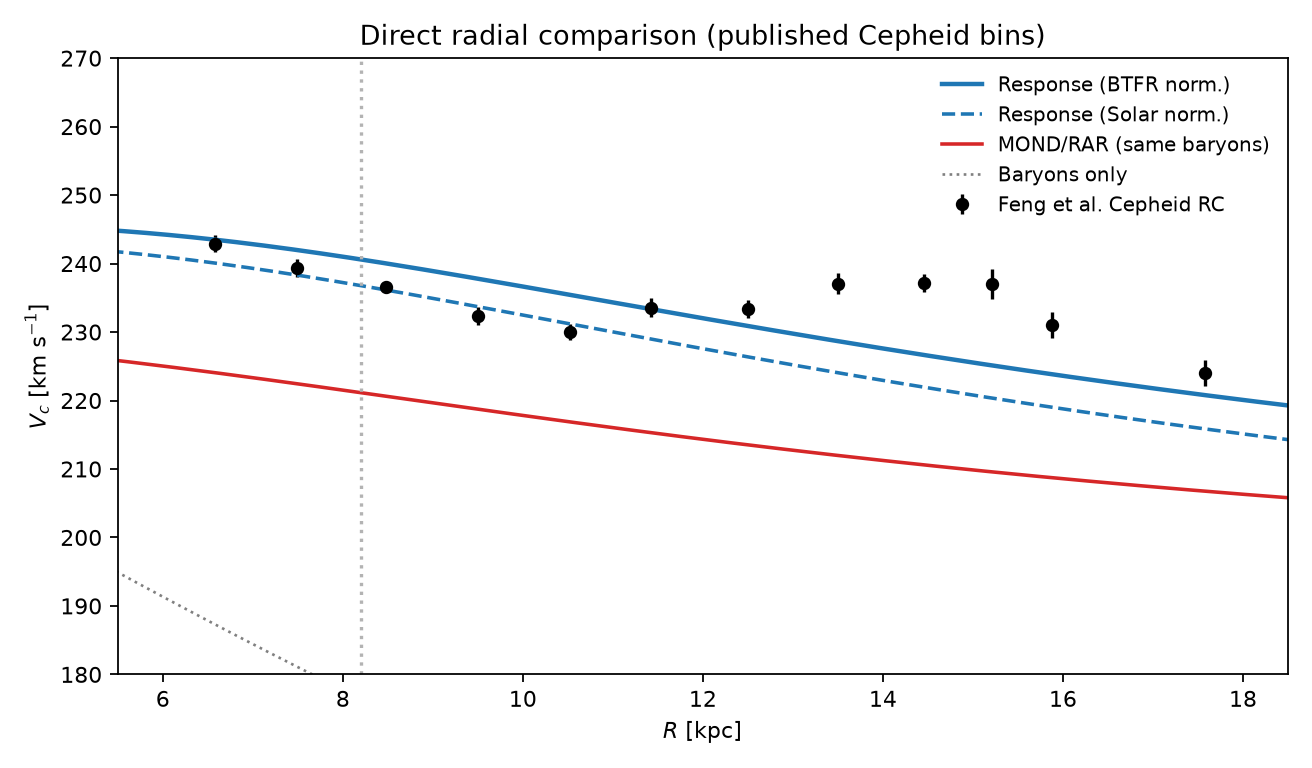
\includegraphics[width=0.88\textwidth]{paper3_gaia_radial_direct_test.png}
\caption{Direct radial comparison with the published Gaia DR3 classical-Cepheid rotation curve of Feng et al.
The response curves use the fixed baryonic realization; the solid response curve uses the BTFR normalization and the dashed curve is normalized to the Solar-circle speed.
The MOND/RAR curve uses the same baryonic acceleration.}
\label{fig:gaiaRC}
\end{figure}
For the quoted bin errors, the BTFR-normalized response realization gives
\begin{equation}
\chi^2=203.7\quad(12\ \text{bins}),\qquad
\mathrm{RMS}(V_{\rm model}-V_{\rm obs})=6.25\,\kms.
\end{equation}
Solar normalization worsens these to
\begin{equation}
\chi^2=367.1,\qquad \mathrm{RMS}=8.99\,\kms,
\end{equation}
because lowering $V_Q$ underpredicts the outer bins while the Cepheid curve remains comparatively flat.
Neither realization is a statistically adequate description of the binned curve under the quoted errors.
In particular, the smooth axisymmetric response does not reproduce the observed dip near $10$--$11\,$kpc and bump near $13$--$15\,$kpc.
This is an important limitation of the present realization.
Possible non-axisymmetric structure, source-profile uncertainty, and correlated observational/systematic errors require separate treatment; none is fitted here.

\section{Quantitative MOND/RAR comparison}
\label{sec:rar}
For comparison we evaluate the empirical radial-acceleration interpolation~\cite{McGaugh2016}
\begin{equation}
g_{\rm RAR}=\frac{g_b}{1-\exp[-\sqrt{g_b/a_0}]},
\end{equation}
using the same baryonic acceleration $g_b=V_b^2/R$.
This comparison isolates the difference between the response transition and the empirical RAR mapping rather than differences in the baryonic mass model.
\begin{figure}[h]
\centering
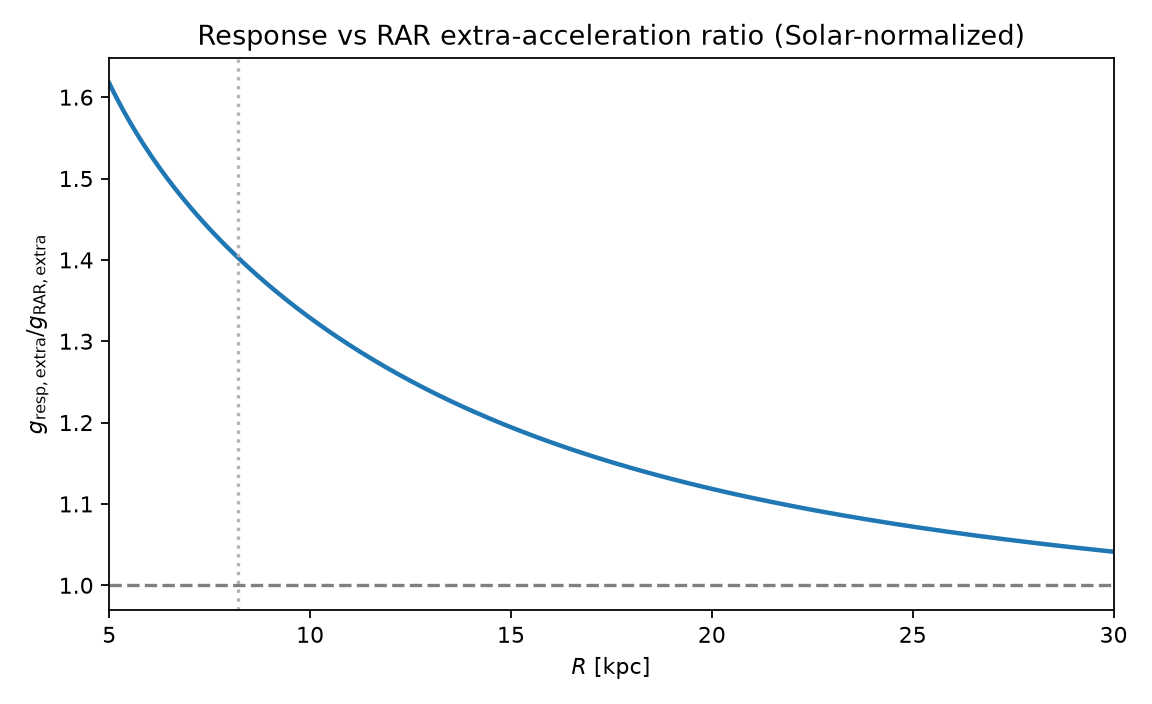
\includegraphics[width=0.84\textwidth]{paper3_response_vs_rar_extra_ratio.png}
\caption{Ratio of the Solar-normalized response acceleration to the extra acceleration implied by the empirical RAR.
The response excess is larger in the inner and intermediate disc and approaches the RAR excess outward.}
\label{fig:rar}
\end{figure}
Across $5$--$30\,$kpc the response excess is about $1.62$ times the RAR excess at $5\,$kpc, $1.40$ times at the Solar circle, and $1.04$ times by $30\,$kpc.
With the present baryonic realization the corresponding MOND/RAR rotation curve is lower than the observed Cepheid curve over much of $6$--$18\,$kpc (Fig.~\ref{fig:gaiaRC}); its 12-bin RMS residual is $20.1\,\kms$.
These numbers are model-specific and should not be read as a general test of MOND: they test this interpolation with this fixed baryonic realization.

\section{Analytic vertical geometry}
\label{sec:vertical-theory}
A localized, centred, axisymmetric planar response source has the far-field carrier density and oblate quadrupole of~\cite{boyd2026galactic}.
A useful local geometric diagnostic is
\begin{definition}[Effective local flattening]
\label{def:qeff-mw}
\begin{equation}
\qeff^{-2}(R)=
\frac{R\,\partial_z^2\Phi(R,0)}{\partial_R\Phi(R,0)}.
\end{equation}
\end{definition}
For a logarithmic oblate potential
\begin{equation}
\Phi_q(R,z)=\frac{V^2}{2}\ln\!\left(R^2+\frac{z^2}{q^2}\right),
\end{equation}
this definition returns the parameter $q$ exactly.
The quadrupole expansion gives
\begin{equation}
\qeff^{-2}(R)=1+\frac{\langle R^2\rangle}{R^2}+O(R^{-4}).
\end{equation}
For an exponential planar source, $\langle R^2\rangle=6R_d^2$, hence
\begin{corollary}[Exponential-disc Solar estimate]
\label{cor:qth}
\begin{equation}
\boxed{\qeff(R)\simeq\left[1+6\left(\frac{R_d}{R}\right)^2\right]^{-1/2}}.
\end{equation}
Taking $R_d=2.5\,$kpc (thin-disc scale) and $R_0=8.2\,$kpc yields
\begin{equation}
\boxed{\qth(R_0)=0.80.}
\end{equation}
\end{corollary}
This is a theoretical estimate from the source geometry, not a fit to Gaia.
Because $R_0/R_d\simeq3.3$, higher multipoles are not parametrically negligible enough to call $0.80$ an exact Solar-radius prediction.
The robust asymptotic statement is $\qeff<1$ for the leading disc quadrupole and $\qeff\to1$ at large radius.

\section{Vertical-geometry experiment}
\label{sec:vertical-exp}
S\"oding et al.~\cite{Soding2025} infer a local dark-matter-equivalent density from Gaia DR3 K dwarfs of
\begin{equation}
\rho_{\rm dm}=0.0117\pm0.0035\,\Msun\,\mathrm{pc}^{-3}.
\end{equation}
We use this as an observational vertical-force constraint, without interpreting the response as particle dark matter.
Paper~2's Poisson closure $\nabla^{2}\Phi_{\mathrm{resp}}=\kappa n$ with an oblate logarithmic response potential
\begin{equation}
\Phi_q(R,z)=\frac{V_{\rm resp}^2}{2}\ln\!\left(R^2+\frac{z^2}{q^2}\right)
\end{equation}
gives the vertical force
\begin{equation}
K_z(R,z)=\frac{V_{\rm resp}^2 z/q^2}{R^2+z^2/q^2},
\end{equation}
and near the plane
\begin{equation}
K_z\simeq\frac{V_{\rm resp}^2}{q^2R_0^2}z
=4\pi G\rho_{\rm eff}z.
\end{equation}
(The last equality is the standard Poisson near-plane identification of an equivalent density.)
Thus
\begin{proposition}[Near-plane equivalent density]
\label{prop:rho-eff}
\begin{equation}
\rho_{\rm eff}(q)=\frac{V_{\rm resp}^2(R_0)}{4\pi Gq^2R_0^2}.
\end{equation}
\end{proposition}
For this experiment we hold the radial response normalization fixed at $V_{\rm resp}(R_0)=157.87\,\kms$, obtained from the measured Solar circular speed and the adopted baryonic contribution.
There are then two distinct quantities:
\begin{align}
\text{theory:}\quad&\qth=0.80,\\
\text{geometric fit:}\quad&\qfit=0.766.
\end{align}
The fitted value matches the central published density; it is not used to generate the theoretical value.

At $q=0.80$ the predicted equivalent density is
\begin{equation}
\boxed{\rho_{\rm eff}=0.01068\,\Msun\,\mathrm{pc}^{-3},}
\end{equation}
which lies $0.29\sigma$ below the published central value.
Mapping the published $1\sigma$ density interval into $q$ gives
\begin{equation}
\boxed{0.672<q<0.915.}
\end{equation}
\begin{figure}[h]
\centering
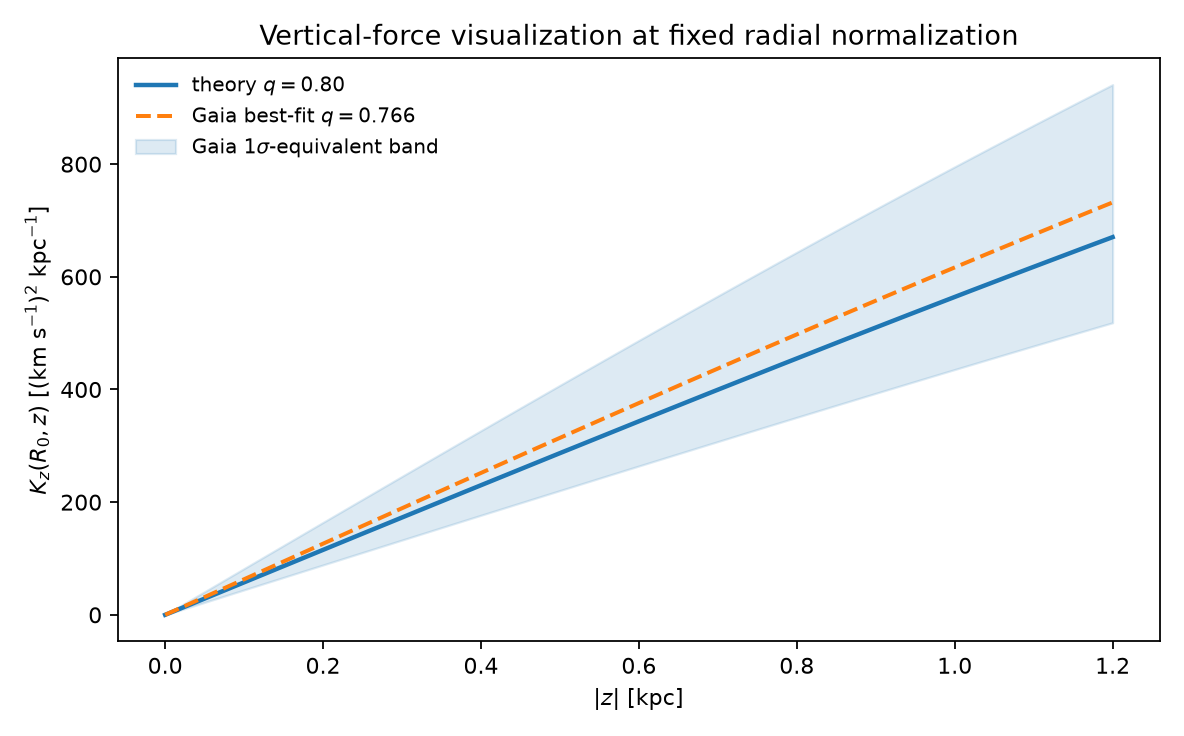
\includegraphics[width=0.86\textwidth]{gaia_q080_theory_vs_bestfit.png}
\caption{Vertical-force visualization.
The solid theoretical curve fixes $q=0.80$ from the leading response quadrupole.
The dashed curve uses the independently fitted $q=0.766$.
The shaded band is the constant-density-equivalent $1\sigma$ range from the published K-dwarf analysis.}
\label{fig:vertical}
\end{figure}
\begin{figure}[h]
\centering
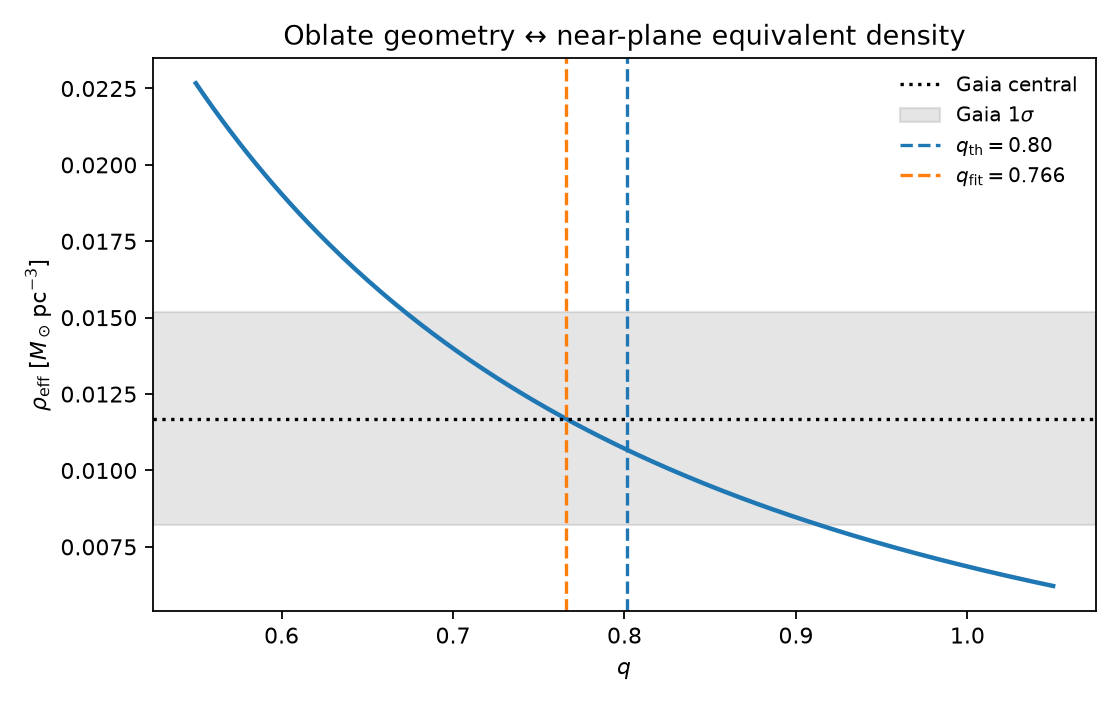
\includegraphics[width=0.82\textwidth]{gaia_q080_density_mapping.png}
\caption{Mapping between oblate response geometry and equivalent near-plane density at fixed radial response normalization.
The theoretical $q=0.80$ and the density-matched fit $q=0.766$ are shown separately.}
\label{fig:qmap}
\end{figure}
The agreement is noteworthy because the two numbers arise from different inputs: $\qth$ from the response-source quadrupole and $\qfit$ from local vertical kinematics.
It is nevertheless a one-galaxy, model-dependent consistency test, not a parameter-free confirmation.
In particular, the K-dwarf inference is sensitive to treatment of the Jeans tilt term; S\"oding et al.\ explicitly identify this as an important systematic.

\section{Logical status of the results}
\label{sec:status}
\begin{center}
\small
\begin{tabular}{@{}p{0.34\linewidth}p{0.58\linewidth}@{}}
\toprule
\textbf{Quantity / claim} & \textbf{Status}\\
\midrule
$g_{\mathrm{resp}}=CQ/r$, BTFR exponent, $\qeff$ quadrupole & Inherited theorems from~\cite{boyd2026galactic} (Lean-checked there).\\
Angular mid-plane identity~\eqref{eq:angular} & Literature hypothesis (\texttt{literature\_axisym\_angular\_kernel}).\\
$g_R=\mathcal C Q(<R)/R$ for thin axisymmetric sources & Radial algebra after that identity (Prop.~\ref{prop:axisym-radial}; Lean).\\
$V_{\rm resp}^2=V_Q^2\mathcal T_d(R/R_d)$ & Literature cumulative kernel + proved enclosed-charge algebra.\\
$V_Q^4=Ga_0\Mb$ & Phenomenological BTFR normalization (physical/empirical input).\\
Baryonic parameters, $V_b(R_0)$ & Observationally motivated inputs; not predicted.\\
Mass-weighted multi-component $\mathcal T(R)$ & Computational realization of the production source.\\
$V_c(R_0)=240.6\,\kms$ & Prediction conditional on baryons + BTFR normalization.\\
$\qth=0.80$ & Leading quadrupole estimate for $R_d=2.5\,$kpc at $R_0$ (Cor.~\ref{cor:qth}).\\
$\qfit=0.766$ & One-parameter geometric match to the published central density.\\
Radial $\chi^2$/RMS vs Feng bins & Direct diagnostic; no radial-shape parameter adjusted.\\
Raw Gaia catalogue re-reduction & Deferred (Remark~\ref{rem:data}).\\
\bottomrule
\end{tabular}
\end{center}

\section{Discussion}
\label{sec:discussion}
The Milky Way realization gives two qualitatively different outcomes.
The vertical test is encouraging: a source-geometry estimate $\qth\simeq0.80$ is close to the independently inferred $\qfit=0.766$ and comfortably inside the density-equivalent $1\sigma$ interval.
This is the cleanest present cross-check of the model because the flattening estimate is not extracted from the vertical measurement.

The radial test is mixed.
The BTFR-normalized model lands within a few $\kms$ of the measured Solar-circle speed and tracks the published Cepheid bins at the $\sim6\,\kms$ RMS level, but it does not fit the detailed $6$--$18\,$kpc structure at the precision of the quoted bin errors.
The observed radial structure is therefore a real target for the model rather than something to be hidden by the Solar-circle comparison.
A next calculation should propagate the full multi-component response source in three dimensions, include finite vertical thickness and finite carrier lifetime, and compare against a covariance-aware likelihood.
Those refinements should be specified before examining whether they improve the radial residuals.

The MOND/RAR comparison also remains informative.
Both frameworks can generate an outer acceleration scale tied to baryons, but their finite-radius mappings differ.
In this Milky Way realization the response model supplies more extra radial acceleration than the standard RAR interpolation through the optical disc.
External-galaxy rotation curves therefore provide a direct way to discriminate the two mappings.

\section{Conclusion}
\label{sec:conclusion}
A fixed Milky Way baryonic realization combined with the Hysterical Response Halo of the companion galactic-modelling paper produces an asymptotically flat radial contribution and an oblate finite-source correction.
The BTFR-normalized radial model predicts $240.6\,\kms$ at the Solar circle, close to the Gaia DR3 value $236.8\pm0.8\,\kms$, and has a 12-bin RMS residual of $6.25\,\kms$ against the published Cepheid curve; it does not reproduce the dip-and-bump structure.
The vertical result is stronger within the present approximations.
The leading exponential-disc quadrupole predicts $\qth\simeq0.80$, while the published K-dwarf density constraint gives a separate geometric fit $\qfit=0.766$ and $1\sigma$-equivalent interval $0.672<q<0.915$.
At the theoretical value the predicted equivalent density is only $0.29\sigma$ from the reported central density.
These results motivate a higher-fidelity three-dimensional response calculation while leaving both the successful and unsuccessful comparisons explicit.

\bibliographystyle{plain}
\bibliography{paper_3_refs}
\end{document}
